\documentclass[journal]{IEEEtran}
\usepackage{amsmath,amssymb}
\usepackage{graphicx}
\usepackage{booktabs}
\usepackage{xcolor}
\usepackage{tikz}
\usetikzlibrary{arrows.meta,positioning,fit}
\usepackage{algorithm}
\usepackage{algpseudocode}
\usepackage{url}
\usepackage{cite}
\usepackage{siunitx}

% Text that can only be written once the experiment campaign has run. Search for \pending before submission.
\newcommand{\pending}[1]{\textcolor{red}{\textit{[#1]}}}
% Figures produced by the notebook's Aggregate cell; a placeholder box until they exist.
\newcommand{\maybegraphic}[2]{\IfFileExists{#1}{\includegraphics[width=#2]{#1}}{%
  \fbox{\parbox{#2}{\centering\vspace{1.5em}\pending{figure pending: #1}\vspace{1.5em}}}}}
\newcommand{\NRuns}{40}
\newcommand{\FullSuccess}{100\%}
\newcommand{\RandomSuccess}{0\%}
\newcommand{\FullSimsToSuccess}{147}
\newcommand{\RandomMedianSims}{353}
\newcommand{\RandomVsFullP}{0.008}
\newcommand{\MinPairP}{0.44}
\newcommand{\AuditN}{3}
\newcommand{\AuditMet}{0}


\begin{document}

\title{Language-Model-Guided Topology Synthesis of Piezoelectric Energy-Harvesting Interfaces with Power Screening and Asynchronous Sizing}

\author{\pending{Author list and affiliations}}

\maketitle

\begin{abstract}
Choosing the structure of a piezoelectric energy-harvesting interface is the step that decides whether a
specification can be met at all, and it is still done by hand. We present a closed-loop synthesis method in
which a large language model (LLM) proposes circuit structures, a circuit simulator evaluates them under
several operating conditions, and the measured results are fed back for the next proposal. Three
mechanisms make the loop practical. First, a physics-based power screen rejects unsized structures that
cannot deliver the load's power at the minimum supply voltage, using short simulations with the storage
node fixed at that voltage; for interfaces whose average output current does not increase with the
storage voltage it is a necessary condition for meeting the minimum-voltage requirement. Second, an
evolution strategy sizes the surviving structures in parallel batches while the model is reasoning, so
the model's latency hides the sizing cost. Third, results are returned to the model with plain-language
diagnoses that name the failing function of the circuit. On a specification that a full-bridge rectifier
fails under all six search conditions, \pending{summarise the main result with the numbers in
Table~\ref{tab:variants}: success rate \FullSuccess{} versus \RandomSuccess{} for a model-free baseline at
the same simulation budget, median \FullSimsToSuccess{} simulations to the first design meeting the
specification, held-out and Monte Carlo results}.
\end{abstract}

\begin{IEEEkeywords}
Analog circuit topology synthesis, large language models, piezoelectric energy harvesting, circuit
sizing, evolution strategies, design automation.
\end{IEEEkeywords}

\section{Introduction}
\IEEEPARstart{A}{} piezoelectric transducer on a vibrating structure delivers a small alternating current
through a large internal capacitance. Turning it into a regulated supply for a sensor node requires an
interface circuit, and the interface's \emph{structure} bounds what it can achieve. A full-bridge
rectifier (FBR) can extract at most $f C_p V_{oc}^2$ from a source with open-circuit amplitude $V_{oc}$,
capacitance $C_p$ and frequency $f$, and much less when diode drops are a sizeable fraction of
$V_{oc}$~\cite{lefeuvre2006comparison}. Synchronized switch harvesting on an inductor
(SSHI)~\cite{guyomar2005sshi}, synchronous charge extraction (SECE)~\cite{lefeuvre2005sece} and
bias-flip rectifiers~\cite{ramadass2010biasflip} raise this limit by adding switches and inductors
whose timing is locked to the vibration. A specification that combines weak excitation, heavy loads and
an upper voltage limit under strong excitation forces the designer to combine such mechanisms, and
choosing which ones is the step that decides feasibility; sizing can only tune a structure that is
already capable.

Automated topology synthesis has a long history for amplifiers. Genetic programming over
building blocks~\cite{mcconaghy2011mojito}, graph composition and decomposition~\cite{meissner2015feats,
zhao2020gctg}, knowledge mining~\cite{jiao2015kmr} and deep reinforcement learning (DRL)~\cite{zhao2022drl}
generate candidate structures and verify them by simulation-in-loop sizing. These methods spend most of
their effort on evaluation: the DRL method of Zhao and Zhang generates $10^4$ or more candidate topologies
per run and relies on a hash table, a symbolic fast-evaluation filter and parallel sizing to bring the
number of sized topologies down to tens~\cite{zhao2022drl}. The policy itself starts without design
knowledge and learns it from rewards within each run.

Large language models carry a broad prior over circuit structures and can reason about why a circuit
fails. Recent work uses them to write netlists or code for analog
circuits~\cite{lai2025analogcoder,chen2024artisan} and to generate topologies of power
converters~\cite{chang2024lamagic}. Two obstacles limit their use as the proposer in a synthesis loop.
Their proposals are structurally unreliable: in a pilot run reported in Section~\ref{sec:pilot}, every
proposal of the model connected a clamp diode backwards. And each proposal takes minutes of reasoning, so
a loop that waits for the model and then sizes each proposal serially is slow.

This paper adapts the evaluation pipeline of simulation-based topology synthesis (structural rules, a
hash table, a fast filter for unsized topologies and feasibility sizing~\cite{zhao2022drl}) to a loop in
which an LLM is the proposer, and applies it to piezoelectric harvesting interfaces. Its contributions
are:
\begin{enumerate}
\item A closed-loop method in which the model proposes \emph{structures} and the program owns values,
the test bench and all measurements, with validation, canonical hashing of structures and feedback
rebuilt from a compact state every round (Section~\ref{sec:method}).
\item A power screen for unsized harvesting interfaces: net power into a storage node fixed at the
minimum supply voltage, from short runs over a few value presets, with a derivation of when it is a
necessary condition for the minimum-voltage requirement (Section~\ref{sec:screen}).
\item Asynchronous sizing by an evolution strategy whose parallel generations run during the model's
reasoning time (Section~\ref{sec:sizing}), and diagnostic feedback that names the failing function of a
circuit (Section~\ref{sec:diag}).
\item An evaluation protocol with held-out operating conditions, Monte Carlo robustness, ablations and a
model-free baseline at an equal simulation budget (Sections~\ref{sec:setup}--\ref{sec:results}).
\end{enumerate}

\section{Related Work}
\emph{Topology synthesis.} Topology-selection methods choose from a library; topology-generation methods
construct circuits from building blocks by genetic operators~\cite{mcconaghy2011mojito} or graph
grammars~\cite{meissner2015feats,zhao2020gctg}; refinement methods modify known circuits using mined
knowledge~\cite{jiao2015kmr}. Zhao and Zhang cast generation as a sequential decision process and train a
policy-gradient network that learns which building block to add~\cite{zhao2022drl}; their evaluation
pipeline (hash table, a symbolic DC-gain filter with a deliberately relaxed threshold, NSGA-II
sizing~\cite{deb2002nsga2} that stops at the first feasible design) is the direct model for ours.
Fast-evaluation filters for unsized topologies were studied in~\cite{zhao2018fast}.

\emph{Learning for circuit design.} Reinforcement learning has been used for
sizing~\cite{settaluri2020autockt} and graph neural networks for predicting circuit
properties~\cite{dong2023cktgnn}. LLM-based approaches generate SPICE netlists or code with simulator
feedback~\cite{lai2025analogcoder}, fine-tune models on amplifier design knowledge~\cite{chen2024artisan},
or generate converter topologies from language descriptions~\cite{chang2024lamagic}.

\emph{Piezoelectric interfaces.} Nonlinear interfaces such as SSHI~\cite{guyomar2005sshi},
SECE~\cite{lefeuvre2005sece} and the bias-flip rectifier~\cite{ramadass2010biasflip} are designed by
hand from an analysis of the charge flow in each half cycle; comparisons such
as~\cite{lefeuvre2006comparison} show that the best structure depends on the excitation and load.

\section{Problem Formulation}\label{sec:problem}
\subsection{Source, load and conditions}
The transducer is modelled as a current source $i_p(t) = I_p\sin(2\pi f t)$ in parallel with $C_p$ and a
\SI{20}{\mega\ohm} leakage resistance, between terminals $p^+$ and $p^-$. The interface must supply a
resistive load $R_L$ from a storage capacitor at node \texttt{out}. Table~\ref{tab:conditions} lists the
ten operating conditions. Six \emph{search} conditions vary load, excitation, frequency, $C_p$ and
temperature; four \emph{held-out} conditions are used only after the search has stopped.

\begin{table}[t]
\centering\footnotesize
\caption{Operating conditions. Held-out conditions are never shown to the model nor used for scoring,
selection or stopping.}\label{tab:conditions}
\resizebox{\columnwidth}{!}{\begin{tabular}{llp{3.2cm}rrrrr}
\toprule
ID & Set & Description & $I_p$ ($\mu$A) & $f$ (Hz) & $C_p$ (nF) & $R_L$ (k$\Omega$) & $T$ ($^\circ$C) \\
\midrule
S1 & search & nominal & 50 & 100 & 25 & 330 & 27 \\
S2 & search & heavy load & 50 & 100 & 25 & 150 & 27 \\
S3 & search & strong excitation, light load & 100 & 100 & 25 & 2200 & 27 \\
S4 & search & weak excitation & 30 & 100 & 25 & 1000 & 27 \\
S5 & search & low frequency & 40 & 80 & 25 & 470 & 27 \\
S6 & search & Cp +20 \%, hot & 50 & 100 & 30 & 330 & 60 \\
H1 & held-out & weak excitation, mid load & 35 & 100 & 25 & 470 & 27 \\
H2 & held-out & high frequency, Cp $-$15 \% & 60 & 120 & 21.25 & 220 & 27 \\
H3 & held-out & very strong excitation, open load, cold & 120 & 100 & 25 & 10000 & -20 \\
H4 & held-out & hot, heavy load & 50 & 100 & 25 & 200 & 85 \\
\bottomrule
\end{tabular}
}
\end{table}

\subsection{Specification}
Every criterion of Table~\ref{tab:criteria} must hold under every condition in a \SI{0.8}{s} transient
that starts from \SI{0}{V}. Together they require the output to stay in a $[1.8, 3.6]$~V window with
small ripple, to start up within \SI{0.4}{s}, and to have settled by the end of the run.

\begin{table}[t]
\centering\footnotesize
\caption{Pass/fail criteria (all conditions).}\label{tab:criteria}
\resizebox{\columnwidth}{!}{\begin{tabular}{llrp{5.2cm}}
\toprule
Criterion & Measure & Requirement & Meaning \\
\midrule
vout\_min & vavg & $\geq$ 1.8 V & settled mean output reaches the load's minimum supply \\
vout\_max & vmax & $\leq$ 3.6 V & output never exceeds the load's absolute maximum \\
ripple & vpp & $\leq$ 0.05 V & peak-to-peak ripple in the final window \\
startup & tup & $\leq$ 0.4 s & cold start: first time output reaches 1.8 V \\
settled & dv & $\leq$ 0.02 V & mean output changes little between the last two windows \\
\bottomrule
\end{tabular}
}
\end{table}

\subsection{Why the specification is hard}
At the nominal condition $V_{oc} = I_p/(2\pi f C_p) \approx \SI{3.2}{V}$. An FBR charging a storage
voltage $V_r$ through two diodes with drop $V_D$ delivers on average
\begin{equation}\label{eq:fbr}
P_{\mathrm{FBR}}(V_r) = 4 f C_p V_r\,(V_{oc} - V_r - 2V_D),
\end{equation}
whose maximum over $V_r$ for $V_D=0$ is $P^\star = f C_p V_{oc}^2 = I_p^2/(4\pi^2 f C_p)$~\cite{lefeuvre2006comparison}.
With Schottky drops of about \SI{0.25}{V}, \eqref{eq:fbr} gives \SI{16}{\micro W} at $V_r=\SI{1.8}{V}$ for
S2, below the \SI{21.6}{\micro W} that a \SI{150}{\kilo\ohm} load draws at \SI{1.8}{V}; under S4
($V_{oc}\approx\SI{1.9}{V} < V_r + 2V_D$) the bridge cannot deliver any current at \SI{1.8}{V}; under S3 the unloaded output rises
towards $V_{oc}-2V_D\approx\SI{5.9}{V}$. Meeting all conditions therefore needs a structure that extracts
more power at low excitation \emph{and} limits the output at high excitation.

\subsection{Design space}
A design is a list of at most 16 components over the vocabulary $\{R, C, L, D, S, \mathrm{SYNC}\}$
connected through named nodes, with reserved nodes \texttt{0}, \texttt{pzp}, \texttt{pzn} and
\texttt{out}. Diodes are a low-drop Schottky, a silicon small-signal diode or a \SI{3.3}{V} zener.
Inductors carry a series resistance of $2\,\Omega + 5\,\Omega$/mH. A switch ($R_{on}=2\,\Omega$) is driven
by a SYNC controller that closes it for $t_{on}$ at the extrema of the piezo voltage (both, positive or
negative), optionally shifted by a phase; each controller draws \SI{0.5}{\micro A} from \texttt{out}.
At most four switches and two controllers are allowed. The controller is an abstraction of the
peak detectors used in SSHI and SECE circuits~\cite{guyomar2005sshi,ramadass2010biasflip}; its timing
is perturbed in the robustness check (Section~\ref{sec:robust}).

\section{Method}\label{sec:method}
Fig.~\ref{fig:flow} shows the loop. Each round, the model receives the specification, the best
structures so far and the results of its previous round, and proposes up to $k$ new structures. Each
new structure is screened, evaluated in full if it passes, and queued for sizing. Sizing runs while the
model reasons about the next round.

\begin{figure}[t]
\centering
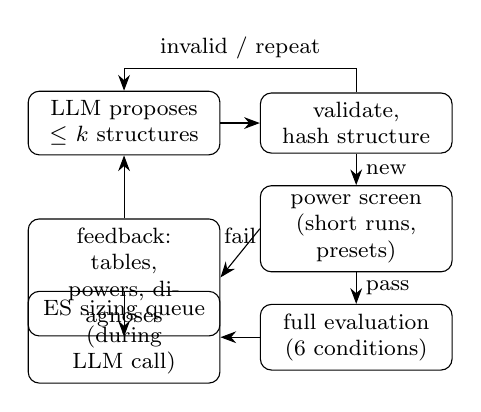
\begin{tikzpicture}[node distance=4mm and 5mm, font=\footnotesize,
  box/.style={draw, rounded corners, align=center, minimum height=7mm, text width=22mm},
  arr/.style={-{Stealth[length=2mm]}}]
\node[box] (llm) {LLM proposes\\ $\le k$ structures};
\node[box, right=of llm] (val) {validate,\\ hash structure};
\node[box, below=of val] (scr) {power screen\\ (short runs,\\ presets)};
\node[box, below=of scr] (full) {full evaluation\\ (6 conditions)};
\node[box, left=of full] (size) {ES sizing queue\\ (during LLM call)};
\node[box, below=of llm, yshift=-4mm] (fb) {feedback: tables,\\ powers, diagnoses};
\draw[arr] (llm) -- (val);
\draw[arr] (val) -- node[right]{new} (scr);
\draw[arr] (scr) -- node[right]{pass} (full);
\draw[arr] (full) -- (size);
\draw[arr] (scr.west) -- node[above]{fail} (fb.east);
\draw[arr] (size) -- (fb);
\draw[arr] (fb) -- (llm);
\draw[arr] (val.north) |- ++(0,3mm) -| node[above, pos=0.25]{invalid / repeat} (llm.north);
\end{tikzpicture}
\caption{The synthesis loop. Held-out conditions and the Monte Carlo check run only after the loop stops.}
\label{fig:flow}
\end{figure}

\subsection{Representation, validation and structure hashing}
The model replies with JSON: a list of proposals, each a list of components with type, nodes and
values, a move label and a rationale. The program adds the piezo model, the load, the controller supply
currents, \SI{1}{\giga\ohm} bleed resistors on all non-ground nodes, the device models and the
measurements, so the model can change connectivity freely but cannot change the test. Validation checks
types, value ranges, controller references, dangling nodes, connectivity between \texttt{out} and the
piezo, component counts, and a rule added after the pilot run: a diode from \texttt{out} to ground is
rejected with a message stating the correct orientation of a clamp. Each structure is reduced to a
canonical form by Weisfeiler--Lehman relabelling~\cite{shervashidze2011wl} of its component--node graph,
with polar pins for diodes and values ignored; its hash identifies repeats, which are not simulated
again whatever their values. Simulations are also cached by the exact netlist text.

\subsection{Power screen for unsized structures}\label{sec:screen}
A full evaluation of one design costs six \SI{0.8}{s} transients. To avoid spending it, and the sizing
that would follow, on structures that cannot work, each new structure first goes through a screen. The
storage node is fixed at $V_s = \SI{1.8}{V}$ by a voltage source behind a \SI{100}{\ohm} sense resistor,
the load is removed, and the net power into the source, $P_{net}(V_s)$, is averaged over the last four
cycles of a ten-cycle run. The controller supply currents remain connected, so $P_{net}$ is net of
their cost.

\emph{Necessary condition.} Let $I(V)$ be the average current an interface delivers into a storage node
held at $V$. Suppose the output can be held at some $V\ge V_s$ in steady state with load $R_L$; then
$I(V) = V/R_L$. If $I$ is non-increasing in $V$, as it is for rectifier-based interfaces including
\eqref{eq:fbr} and the SSHI family, then $I(V_s) \ge I(V) = V/R_L \ge V_s/R_L$, so
\begin{equation}\label{eq:screen}
P_{net}(V_s) = V_s I(V_s) \;\ge\; V_s^2/R_L .
\end{equation}
A structure violating \eqref{eq:screen} on any condition therefore fails the minimum-voltage criterion
there, whatever its storage capacitor. The screen tests \eqref{eq:screen} on the three conditions with
the highest demand relative to supply (S2, S4, S6).

\emph{Relaxation and presets.} The structure's values are untuned at this point, so the screen evaluates
up to four value presets: the proposed values; for every structure with a controller and an inductor,
$t_{on} = \pi\sqrt{L C_p}$ (a half resonance period of the inductor with the nominal $C_p$, which inverts
the piezo voltage) and half of it; and random log-uniform perturbations within a factor of three. A
structure passes if its best preset reaches $\alpha = 0.5$ of the right-hand side of \eqref{eq:screen} on
every screen condition. As with the relaxed DC-gain threshold of~\cite{zhao2022drl}, $\alpha<1$ trades a
few unnecessary evaluations for fewer wrong rejections; the \texttt{audit} variant measures the rate of
wrong rejections (Section~\ref{sec:audit}). One screen costs $3\times 4$ runs of $10/f$, about one
eighth of a full evaluation, and the best preset becomes the starting point of sizing. The screen also
yields a figure of merit, $P_{net}(V_s)/P^\star$, the power relative to the ideal-bridge maximum.

\subsection{Asynchronous sizing}\label{sec:sizing}
Structures that pass the screen are evaluated in full and queued for sizing by an elitist $(1+\lambda)$
evolution strategy~\cite{rechenberg1973,hansen2016cma} over all numeric parameters, in logarithmic
coordinates for $R$, $C$, $L$ and $t_{on}$ and additive coordinates for phase
(Algorithm~\ref{alg:es}). Each generation of $\lambda=8$ designs is simulated as one batch of
$8\times 6$ parallel transients. The step size grows by 1.3 after a generation that improves the
parent and shrinks by 0.82 otherwise, a success rule in the spirit of~\cite{rechenberg1973}. A sizer
stops when its parent meets the specification (feasibility, as in~\cite{zhao2022drl}), when it has used
its budget of 48 evaluations, or when the step size falls below 0.02. Sizers are resumable: while the
model is reasoning, the loop repeatedly advances the unfinished sizer with the best parent, so the
model's latency (minutes per call) pays for the sizing. After the last round the two best unfinished
structures are sized to completion. Structures whose output never exceeds \SI{0.9}{V} are not sized,
because no choice of values fixes a wiring error.

\begin{algorithm}[t]
\caption{Resumable $(1+\lambda)$-ES sizing step}\label{alg:es}
\begin{algorithmic}[1]
\Require parent $x$ with evaluation $e$, step $\sigma$, budget $B$, evaluations used $n$
\State $X \gets$ up to $\min(\lambda, B-n)$ new designs: $x_i \gets x \odot \exp(\sigma z)$, $z\sim\mathcal{N}(0,I)$ (phase: $+0.1\sigma z$), clamped to the limits
\State $E \gets$ evaluate all of $X$ on the search conditions in one parallel batch
\If{some $x_i$ is better than $x$} \State $x, e \gets$ best of $X$; $\sigma \gets 1.3\sigma$
\Else \State $\sigma \gets 0.82\sigma$ \EndIf
\State $n \gets n + |X|$; stop if $e$ meets the specification, $n\ge B$ or $\sigma < 0.02$
\end{algorithmic}
\end{algorithm}

\subsection{Scoring and selection}
Each check yields a margin $m = (y - \ell)/s$ for a measurement $y$, limit $\ell$ and scale $s$ (sign
chosen so that $m\ge 0$ passes; a missing measurement counts as $m=-1$). The score of a design is
$10\,n_{c} + n_{k} + \sum \min(0,\max(m,-1)) + 0.05\sum \min(\max(m,0),0.5)$, where $n_c$ counts conditions
with every check passed and $n_k$ checks passed; ties go to fewer components. The selected design is the
best on the search conditions, the reference included.

\subsection{Feedback to the model}\label{sec:diag}
Prompts are rebuilt every round from a compact state rather than accumulated: the specification and
reference results (system prompt), the four best structures with their sized values, per-condition
tables, screen powers and sizing status, every result of the previous round (invalid, repeated, rejected
by the screen with its powers, or evaluated), and the list of structures explored. Each result also
carries \emph{diagnoses} derived from the measurements: an output that never exceeds \SI{0.9}{V} (with the
note that something may conduct from \texttt{out} to ground), insufficient power on named conditions,
overvoltage, slow start, drift, ripple, or simulation failure. Diagnoses name the symptom and the
function that fails, not a remedy, so that they do not steer the model toward a known topology. If the
last three designs share a major diagnosis, the prompt says so explicitly.

\subsection{Stopping, held-out check and robustness}\label{sec:robust}
The loop stops at the first of: a design meeting the specification on the search conditions; the model
declaring that no structural change can help; three failed model calls; five rounds without improving
the best proposed design; or the wall-clock, simulation or round budget. Then the selected design and
the reference are evaluated once on the held-out conditions, and the selected design is simulated on all
ten conditions for 16 Monte Carlo samples with $R$ $\pm$5\,\%, $C$ $\pm$20\,\%, $L$ $\pm$10\,\%,
$t_{on}$ $\pm$5\,\% and switch timing $\pm$2\,\% of a period (uniform).

\section{Experimental Setup}\label{sec:setup}
The proposer is Gemma~4 31B~\cite{gemma4} served by vLLM, with reasoning enabled and temperature 1.0;
repairs of unusable replies use one call without reasoning. Simulations use LTspice~\cite{ltspice} in
batch mode under Wine, eight in parallel, with a \SI{2}{\micro s} maximum time step. Each run has a budget
of 12 rounds of up to $k=3$ proposals, \SI{1}{h} of wall-clock time and 3000 simulations. We compare the
variants in Table~\ref{tab:variants}, each over five seeds: the full method; without the screen; without
diagnoses; one proposal per round (with 24 rounds); coordinate search instead of the evolution strategy;
without model reasoning; and a model-free baseline that proposes random valid circuits over the same
vocabulary through the same screen and sizing. The \texttt{audit} variant equals the full method but also
sizes every structure the screen rejects, outside selection. Because all variants share a simulation
budget, they are compared by the number of simulations used, which does not depend on the load of the
shared model server; wall-clock times are reported for completeness. Metrics are the fraction of runs
meeting the specification on the search conditions and on all conditions, the number of simulations
and minutes until the first design meeting the specification, the fraction of invalid proposals, and the
Monte Carlo pass rate of the selected design.

\section{Results}\label{sec:results}
\subsection{Pilot run and calibration}\label{sec:pilot}
A smoke test simulated the reference FBR (four Schottky diodes, \SI{2.2}{\micro F}) and a hand-designed
witness (parallel SSHI with \SI{4.7}{mH}, $t_{on}=\SI{34}{\micro s}$, the FBR and a \SI{3.3}{V} zener
clamp), which is never shown to the model. The reference failed all six search conditions: its mean
output was \SI{1.76}{V} under S2 and \SI{1.51}{V} under S4, consistent with \eqref{eq:fbr}, and it reached
\SI{5.7}{V} under S3; at S1 and S5 it met the voltage window but had not settled by \SI{0.8}{s}. The
witness met every criterion on all six search conditions, so the specification is feasible. The smoke
test also exposed a modelling error: without temperature parameters the Schottky model took silicon
defaults, its saturation current at \SI{85}{\celsius} became comparable to the piezo current, and both circuits
collapsed under H4. The model was corrected (Schottky barrier height and saturation-current exponent)
before all runs reported below; Table~\ref{tab:reference} gives the reference and witness under the
corrected models.

\begin{table}[t]
\centering\footnotesize
\caption{Reference (FBR) and witness on every condition: mean and peak output and overall verdict.}\label{tab:reference}
\resizebox{\columnwidth}{!}{\begin{tabular}{l rrl rrl}
\toprule
Cond. & FBR $\bar V$ & FBR $V_{max}$ & FBR & Witness $\bar V$ & Witness $V_{max}$ & Witness \\
\midrule
S1 & 2.24 & 2.25 & fail & 3.38 & 3.38 & pass \\
S2 & 1.76 & 1.77 & fail & 3.35 & 3.36 & pass \\
S3 & 5.68 & 5.72 & fail & 3.40 & 3.42 & pass \\
S4 & 1.51 & 1.52 & fail & 3.37 & 3.37 & pass \\
S5 & 2.26 & 2.28 & fail & 3.37 & 3.38 & pass \\
S6 & 1.93 & 1.94 & pass & 3.38 & 3.39 & pass \\
H1 & 1.63 & 1.64 & fail & 3.37 & 3.37 & pass \\
H2 & 2.41 & 2.42 & pass & 3.38 & 3.38 & pass \\
H3 & 6.90 & 6.95 & fail & 3.39 & 3.40 & pass \\
H4 & 1.55 & 1.56 & fail & 3.34 & 3.35 & fail \\
\bottomrule
\end{tabular}
}
\end{table}

A pilot search with an earlier version of the loop (one proposal per call, no screen, no diagnoses,
coordinate-search tuning) is instructive. Each model call took \SIrange{110}{220}{s} with 4.6k--8.7k
completion tokens. The model proposed sensible structures by name (parallel SSHI with a clamp, SECE,
a synchronous switched bridge), but all four distinct proposals connected the \SI{3.3}{V} zener with its
anode at the output, which forward-biases it and pins the output near \SI{0.66}{V}; one also reversed the
bridge's return diodes. No output exceeded about \SI{0.7}{V} on any condition, value tuning could not
change that (three of the four scores did not move at all), and the run stopped on stagnation after
\SI{20}{min}, returning the reference. Two lessons shaped the method: structural
errors of a predictable kind should be caught by validation and named in the feedback, and effort spent
sizing a structure that cannot work should be avoided, which the screen and the \SI{0.9}{V} rule do.

\subsection{Comparison of variants}
Table~\ref{tab:variants} and Fig.~\ref{fig:variants} summarise \NRuns{} runs.
\pending{Describe the comparison once the campaign has run: success rates of the full method against the
random baseline and each ablation; the simulations to first success; which mechanism contributes most;
the invalid-proposal rate with and without diagnoses. State differences only where the five seeds
support them, and report the spread.}

\begin{table*}[t]
\centering\footnotesize
\caption{Variants over five seeds at an equal budget of 3000 simulations. ``Spec met'': runs whose selected
design meets every criterion on the six search conditions; ``+held-out'': also on the four held-out
conditions; simulations and minutes to success: medians over successful runs; ``Invalid'': proposals
rejected by validation; ``MC pass'': median Monte Carlo pass rate of the selected design.}\label{tab:variants}
\begin{tabular}{lrrrrrrrr}
\toprule
Variant & Runs & Spec met & +held-out & Sims to success & Min to success & Sims & Invalid & MC pass \\
\midrule
full & 5 & 100\% & 20\% & 147 [27--291] & 7 & 315 & 8\% & 50\% \\
no\_screen & 5 & 100\% & 0\% & 156 [12--558] & 7 & 324 & 8\% & 0\% \\
no\_diag & 5 & 100\% & 40\% & 27 [27--303] & 7 & 195 & 0\% & 25\% \\
single & 5 & 100\% & 40\% & 237 [27--699] & 9 & 405 & 0\% & 31\% \\
coord & 5 & 100\% & 40\% & 27 [27--87] & 5 & 195 & 0\% & 38\% \\
no\_think & 5 & 100\% & 0\% & 165 [87--549] & 4 & 333 & 11\% & 6\% \\
random & 5 & 0\% & 0\% & -- & -- & 353 & 0\% & 0\% \\
audit & 5 & 100\% & 20\% & 27 [27--1251] & 7 & 195 & 0\% & 31\% \\
\bottomrule
\end{tabular}

\end{table*}

\begin{figure}[t]
\centering
\maybegraphic{generated/fig_variants.pdf}{\columnwidth}
\caption{Fraction of runs meeting the specification (left) and simulations until the first design that
meets it (right), per variant.}\label{fig:variants}
\end{figure}

\subsection{How often does the screen reject a workable structure?}\label{sec:audit}
In the \texttt{audit} variant every structure rejected by the screen was evaluated and sized with the
same budget, outside selection. Table~\ref{tab:audit} reports how many of them still met the
specification. \pending{Interpret: the fraction of correct rejections and what it implies for $\alpha$;
compare with the 99\,\% correct rejections of the relaxed DC-gain filter in~\cite{zhao2022drl}.}

\begin{table}[t]
\centering\footnotesize
\caption{Screen audit: structures rejected by the screen and sized anyway.}\label{tab:audit}
\begin{tabular}{rrr}
\toprule
Rejected and audited & Met spec after sizing & Correct rejections \\
\midrule
3 & 0 & 100\% \\
\bottomrule
\end{tabular}

\end{table}

\subsection{Synthesized designs}
\pending{Show the structure of the best design from the full method (schematic), its per-condition
results against the reference, its held-out results, its power gain over the ideal bridge from the
screen ($P_{net}/P^\star$) and its Monte Carlo pass rate by condition. Discuss whether the model recombined
known mechanisms (e.g.\ SSHI with a clamp) or proposed a structure not in the cited literature.}

\begin{figure}[t]
\centering
\maybegraphic{generated/fig_progress.pdf}{\columnwidth}
\caption{Score of every design evaluated in a representative run of the full method; proposals in
colour, sizing steps in grey, best so far in black.}\label{fig:progress}
\end{figure}

\subsection{Cost}
\pending{Report median wall time, model time, tokens per run and simulations per run for the full method;
the share of simulations spent on screening, full evaluations and sizing; and the fraction of sizing
that overlapped model calls.}

\section{Discussion}
\emph{What the language model contributes.} The model supplies structures from a prior that includes
the literature on nonlinear piezo interfaces. That makes it efficient on specifications whose solution
recombines known mechanisms, which is the case here, and the random baseline quantifies how much this
prior is worth at equal simulation cost. It also means that success on this specification does not show
that the method invents new structures; a benchmark whose solutions are not in the literature would be
needed for that claim.

\emph{Comparison with DRL synthesis.} The DRL method of~\cite{zhao2022drl} learns a policy from scratch
within each run and needs thousands of episodes; once trained, it returns a solution for the same
specification immediately. The LLM-based loop needs no training and few proposals but pays minutes per
proposal and has no memory across runs. The domains (amplifiers there, harvesting interfaces here) and
the evaluation stacks differ, so we do not compare numbers directly.

\emph{Threats to validity.} The controller is ideal apart from the timing perturbation of the Monte
Carlo check; real peak detectors add delay and start-up power. Device models are generic and there is no
mechanical coupling: the piezo current does not depend on the electrical load, which favours
interfaces that would damp a real resonator. The screen's necessary-condition argument assumes an
average output current that does not increase with the storage voltage; structures that violate it
could be rejected wrongly, which the audit measures. The model is not deterministic and is served on a
shared cluster, so we report medians over seeds and compare by simulations rather than time. The
specification was set by the authors and checked only for feasibility with one witness circuit.

\section{Conclusion}
We presented a closed-loop method in which a language model proposes the structures of piezoelectric
harvesting interfaces and a simulation pipeline (validation, structure hashing, a power screen for
unsized structures, asynchronous evolution-strategy sizing and diagnostic feedback) turns the proposals
into verified, sized designs, checked on held-out conditions and under component tolerances.
\pending{State the main quantitative result.} Future work includes a benchmark of specifications whose
solutions are not textbook circuits, realistic controller and transducer models, and sharing learned
structures across runs.

\bibliographystyle{IEEEtran}
\bibliography{refs}

\end{document}
